\chapter{Theoretical Foundation}

\section{Machine Learning}

\begin{enumerate}
    \item Loss Function / Error Metrics
    \item Supervised --- Unsupervised / Categorization
    \item Optimization techniques: Stochastic-Batch Gradient Descent, GD Momentum, Adam
    \item Bias-Variance tradeoff / Overfitting --- Underfitting
\end{enumerate}

\section{Deep Learning}
\begin{enumerate}
    \item ANN / MLP % Node, Feedforward, Backpropagation / Optimization
        \begin{itemize}
            \item Architecture $\rightarrow$ Input, Hidden, Output
            \item Feedforward
            \item Optimization $\rightarrow$ Backpropagation, SGD, ADAM, \ldots
        \end{itemize}
    \item Regularization
    \item important architectures
        \begin{itemize}
            \item CNN % layers --- convolutional, max-pooling
            \item RNN % recurrent layer
            \item Specific foundation architectures for relevant approaches
        \end{itemize}
\end{enumerate}

\textbf{Deep Learning in Character Recognition Considering Pattern Invariance
Constraints}~\cite{oyedotun_deep_2015}
Deep Learning: neural network architecture of more than a single hidden layer as opposed to shallow networks
Features of deep networks: distributed representation of knowledge at each hidden layer, distinct
features are extracted by units or neurons in each hidden layer
several units can be active concurrently
Each layer extracts moredefined/advanced features $\rightarrow$ hierarchical representation of
features

Common problems with training deep learning
\begin{itemize}
    \item saturating units
    \item vanishing gradients
    \item over-fitting \& underfitting
\end{itemize}

Classification of deep learning architectures
\begin{itemize}
    \item Generative Architectures:\\
        not deterministic of class patterns that input belong to $\rightarrow$ sample joint
        statistical distribution of data\\
        unsupervised learning: greedy layer-wise pre-training\\
        Use auto encoders (generative) when a lot unlabelled but not a lot labelled data
        $\rightarrow$ generatively train network and then fine tune with labelled
    \item Discriminative Architectures:\\
        required to be deterministic of correlation of input data to the classes of patterns therein\\
        supervised learning
    \item Hybrid\\
        combination of discriminative and generative\\
        generally pre-trained and discriminately fine-tuned for deterministic purposes
\end{itemize}


\textbf{Ohne Quelle}
Generative and Convolution for `feature generation' $\rightarrow$ which one is best?



\subsection{Generative Architectures}
\textbf{Deep Learning in Character Recognition Considering Pattern Invariance
Constraints}~\cite{oyedotun_deep_2015}
Stacked Denoizing Auto Encoder lowest error rate on translation
Deep Belief Network lowest error rate on rotation, scale, low noise

\subsubsection{Auto-Encoder}
Auto-Encoder not always seen as generative!
\textbf{Deep Learning in Character Recognition Considering Pattern Invariance
Constraints}~\cite{oyedotun_deep_2015}
denoizing
\begin{itemize}
    \item Generative
    \item Learn underlying features during training
    \item Single layer, feedfoward network
        \begin{itemize}
            \item input and output neurons in equal amount
            \item number of hidden units is smaller
            \item endcode --- input $\rightarrow$ hidden; decode --- hidden $\rightarrow$ output
        \end{itemize}
    \item Unsupervised (see source for details)
    \item auto encoders can be stacked on one another $\rightarrow$ more distributed and hierarchical
        representation $\rightarrow$ Stacked Auto Encoders
\end{itemize}

\subsubsection{Deep belief network}
\textbf{Deep Learning in Character Recognition Considering Pattern Invariance
Constraints}~\cite{oyedotun_deep_2015}
\begin{itemize}
    \item Generative
    \item graphical and probabilistic, directed acyclic graph composed of stochastic variables
    \item combination of Sigmoid Belief Network (aka Bayesian network) and a Restricted Blotzman Machine
\end{itemize}


\subsection{Convolutional Neural Network}
\textbf{Comparative analysis of deep learning image detection
algorithms}~\cite{srivastava_comparative_2021}
These layers apply filters to extract patterns from images. The filter moves over the image to generates the output. Different filters recognize different patterns. Initial layers have filters to recognize simple patterns. They become more complex through the layers over time as follows:

\textbf{Review of Deep Learning Algorithms and Architectures}~\cite{shrestha_review_2019}
Def Neural Network:
\begin{itemize}
    \item Machine Learning technique that consists of processing units organized in input,
        hidden and output layers
    \item the nodes or units in each layer are connected to nodes in adjacent layers
    \item each connection has weight value
    \item inputs are multiplied by weight and summed up at each unit
    \item the sum is used with an activation function (e.g. ReLU, Sigmoid, Tanh, SoftPlus)
\end{itemize}

\section{Opical Character Recognition}

\textbf{Deep Learning based OCR}~\cite{zhao_improving_2020}
What is OCR:\ process of converting images of typed, handwritten or printed text into machine-encoded one
includes two sub frameworks: text detection and text recognition (based on position coordinates)
\textbf{End-To-End also possible}
Process can include image processing!!!


\textbf{no source}
grid: divides image into parts $\rightarrow$ each part has own bounding boxes
bounding boxes:~regressor for box, each bounding box is assigned an anchor box (respective to grid cell)
anchor boxes:~default `shape' for bounding box

bounding boxes different stages of convolution / 2-d size $\rightarrow$ different object size to detect

\subsection{Text detection}
subfield of object detection (e.g. YOLOv4 can be used for text)

Detect position coordinates containing text in input image
Text detection more challenging

Two object detection methods --- CNN-based
\begin{itemize}
    \item Region-based \\
        views detection problem as classification problem\\
        CNN to extract deep features of proposals by selective search $\rightarrow$  Use SVM to
            classify with features\\
        e.g. R-CNN
    \item  single `look'
        extract feature maps on entire image\\
        directly regress bounding boxes on feature maps\\
        e.g. YOLO --- You Only Look Once, SSD --- Single Shot Detection
\end{itemize}
Non CNN-based: DETR

\subsubsection*{Comparison Object Detection basic algos}
\textbf{Comparative analysis of deep learning image detection
algorithms}~\cite{srivastava_comparative_2021}
YOLO-V3 outperforms SSD and Faster R-CNN

VGG-16 widely used feature generating architecture

\subsubsection*{Faster-RCNN}
A deeper look at how Faster-RCNN works~\cite{goswami_deeper_2018}
composed of 3 neural nets:
\begin{itemize}
    \item Feature Network: pre-trained image classification netork $\rightarrow$ generate good features
    \item Region Proposal Network:
        \begin{itemize}
            \item NN with 3 conv layers
            \item one layer splits up network to: classification and bounding box regression
            \item bounding box regression $\rightarrow$ bounding boxes are region of interes (ROI)
                that might contain an object
        \end{itemize}
    \item Detection Network: take input from previous nets, generate final class and bounding box,
        4 fully connected, 2 stacked common layers shared by classification and bounding box regression
        layer \end{itemize}

\textbf{Deep Learning in Character Recognition Considering Pattern Invariance
Constraints}~\cite{oyedotun_deep_2015}
Neural networks can learn features of task on which they are designed and trained
Neural networks better than other approaches (e.g.\ template matching, syntactic analysis)
$\rightarrow$ NNs can learn and adapt to moderate variations (e.g.\ translation, rotation, scaling,
noisy patterns)

\subsection{Character recognition}
Recognize text based on position coordinates
\begin{center}
    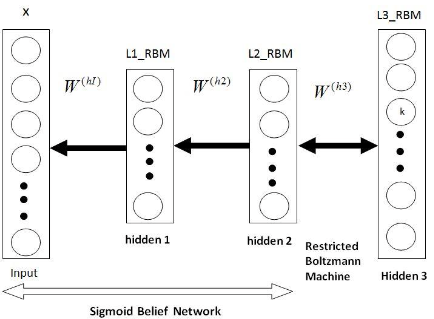
\includegraphics[width=\textwidth]{img/Deep-Belief-Network.png}
\end{center}

\subsection{End-To-End}
